\documentclass[12pt, a4paper]{article}
\usepackage[utf8]{inputenc}
\usepackage{amsmath}
\usepackage{amsthm}
\usepackage{amssymb}
\usepackage{graphicx}
\usepackage{parskip}
\usepackage{hyperref}
\usepackage{fancyhdr}
\usepackage{lastpage}
\usepackage[vlined,ruled]{algorithm2e}
\usepackage[acronym]{glossaries}
\usepackage{caption}
\usepackage{titlesec}
\usepackage{tikz}
\usetikzlibrary{arrows,automata}

\titleformat{\section}
  {\normalfont\bfseries}{Problem 3.\thesection}
  {0em}{}

\titleformat{\subsection}
  {\normalfont\bfseries}{3.\thesubsection}
  {0em}{}
  
\titleformat{\subsubsection}
  {\normalfont\bfseries}{3.\thesubsection}
  {0em}{}

\title{%
  Stochastic Network Modeling \\
  Homework 3 - Solutions
}
\author{%
  Juan Pablo Royo Sales\\
  \small{Universitat Politècnica de Catalunya}
}
\date\today

\pagestyle{fancy}
\fancyhf{}
\fancyhead[C]{}
\fancyhead[R]{Juan Pablo Royo Sales - UPC MIRI}
\fancyhead[L]{SNM - Homework 3}
\fancyfoot[L,C]{}
\fancyfoot[R]{Page \thepage{} of \pageref{LastPage}}
\setlength{\headheight}{15pt}
\renewcommand{\headrulewidth}{0.4pt}
\renewcommand{\footrulewidth}{0.4pt}

\renewcommand{\qedsymbol}{$\blacksquare$}
\newacronym{bpp}{BPP}{BPP}

\begin{document}

\maketitle

\section{}
\subsection{}

\begin{subequations}
  \begin{align}
    P(X(0),X(1),X(2)) &= P(X(1) \cap X(2))\\
                      &= P(X(1))P(X(2))\\
                      &= (p+q)(p+q)\\
                      &= p^2 + 2pq + q^2
  \end{align}
\end{subequations}

\subsection{}

\begin{subequations}
  \begin{align}
    P(X(2)=a) = qq\\
    P(X(2)=b) = 0\\
    P(X(2)=c) = qp + pq = 2pq\\
    P(X(2)=d) = 0\\
    P(X(2)=e) = pp\\
  \end{align}
\end{subequations}

\section{}
\subsection{}
\subsubsection{(a)}
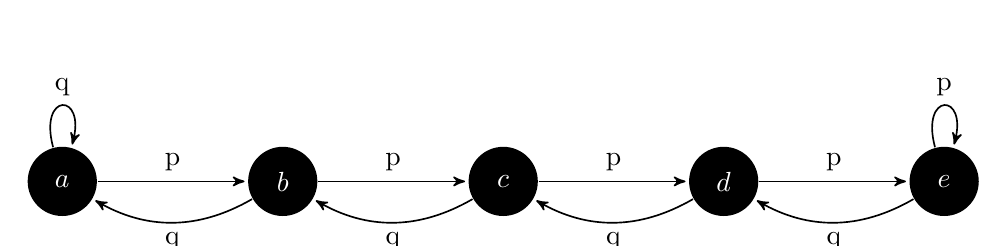
\begin{tikzpicture}[->,>=stealth',shorten >=1pt,auto,node distance=2.8cm,
  semithick]
  \tikzstyle{every state}=[fill=black,draw=none,text=white]

  \node[state]         (A)              {$a$};
  \node[state]         (B) [right of=A] {$b$};
  \node[state]         (C) [right of=B] {$c$};
  \node[state]         (D) [right of=C] {$d$};
  \node[state]         (E) [right of=D] {$e$};

  \path (A) edge [loop above] node {q} (A)
            edge              node {p} (B)
        (B) edge              node {p} (C)
        (B) edge [bend left]  node {q} (A)
        (C) edge              node {p} (D)
        (C) edge [bend left]  node {q} (B)
        (D) edge              node {p} (E)
        (D) edge [bend left]  node {q} (C)
        (E) edge [loop above] node {p} (E)
        (E) edge [bend left]  node {q} (D);
\end{tikzpicture}

\subsubsection{(b)}
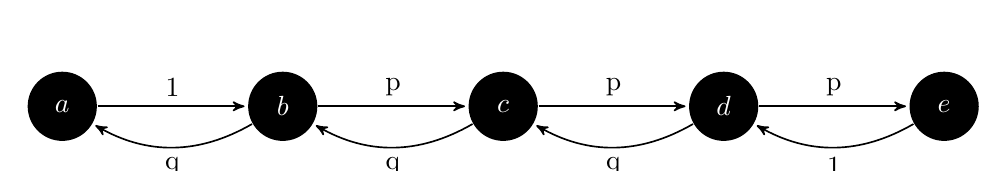
\begin{tikzpicture}[->,>=stealth',shorten >=1pt,auto,node distance=2.8cm,
  semithick]
  \tikzstyle{every state}=[fill=black,draw=none,text=white]

  \node[state]         (A)              {$a$};
  \node[state]         (B) [right of=A] {$b$};
  \node[state]         (C) [right of=B] {$c$};
  \node[state]         (D) [right of=C] {$d$};
  \node[state]         (E) [right of=D] {$e$};

  \path (A) edge              node {1} (B)
        (B) edge              node {p} (C)
        (B) edge [bend left]  node {q} (A)
        (C) edge              node {p} (D)
        (C) edge [bend left]  node {q} (B)
        (D) edge              node {p} (E)
        (D) edge [bend left]  node {q} (C)
        (E) edge [bend left]  node {1} (D);
\end{tikzpicture}

\subsubsection{(c)}
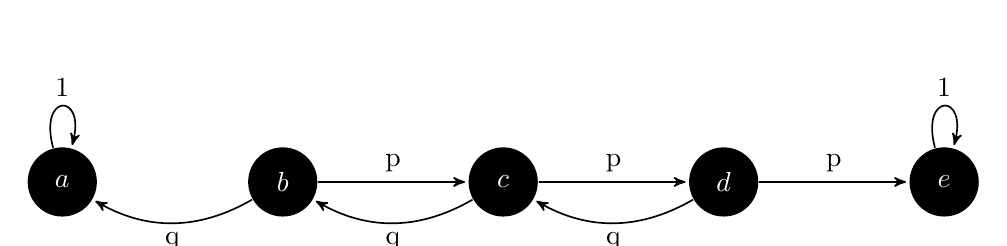
\begin{tikzpicture}[->,>=stealth',shorten >=1pt,auto,node distance=2.8cm,
  semithick]
  \tikzstyle{every state}=[fill=black,draw=none,text=white]

  \node[state]         (A)              {$a$};
  \node[state]         (B) [right of=A] {$b$};
  \node[state]         (C) [right of=B] {$c$};
  \node[state]         (D) [right of=C] {$d$};
  \node[state]         (E) [right of=D] {$e$};

  \path (A) edge [loop above] node {1} (A)
        (B) edge              node {p} (C)
        (B) edge [bend left]  node {q} (A)
        (C) edge              node {p} (D)
        (C) edge [bend left]  node {q} (B)
        (D) edge              node {p} (E)
        (D) edge [bend left]  node {q} (C)
        (E) edge [loop above] node {1} (E);
\end{tikzpicture}

\subsection{}
\subsubsection{(a)}

\begin{align*}
  P = \begin{bmatrix}
    q & p & 0 & 0 & 0\\
    q & 0 & p & 0 & 0\\
    0 & q & 0 & p & 0\\
    0 & 0 & q & 0 & p\\
    0 & 0 & 0 & q & p
  \end{bmatrix}
\end{align*}

\subsubsection{(b)}

\begin{align*}
  P = \begin{bmatrix}
    0 & 1 & 0 & 0 & 0\\
    q & 0 & p & 0 & 0\\
    0 & q & 0 & p & 0\\
    0 & 0 & q & 0 & p\\
    0 & 0 & 0 & 1 & 0
  \end{bmatrix}
\end{align*}

\subsubsection{(c)}

\begin{align*}
  P = \begin{bmatrix}
    1 & 0 & 0 & 0 & 0\\
    q & 0 & p & 0 & 0\\
    0 & q & 0 & p & 0\\
    0 & 0 & q & 0 & p\\
    0 & 0 & 0 & 0 & 1
  \end{bmatrix}
\end{align*}

\section{}
\subsection{}
It is not a $MC$ because the $\sum_j p_{ij} > 1$.
\subsection{}
I think it is possible because we use that extra state to go back from $a$ to $a'$, then from $a'$ to $a$ again and after to $b$.
The same for the case of $e$.

\section{}
\subsection{}

Let $0$ be the Initial State or Loosing.\\
Let $2$ be the state to get $2$ equal dice.\\
Let $3$ be the state to get $3$ equal dice.

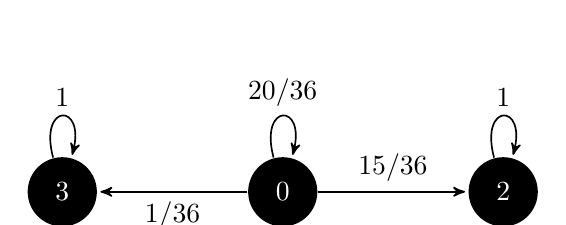
\begin{tikzpicture}[->,>=stealth',shorten >=1pt,auto,node distance=2.8cm,
  semithick]
  \tikzstyle{every state}=[fill=black,draw=none,text=white]

  \node[state]         (A)              {$0$};
  \node[state]         (B) [right of=A] {$2$};
  \node[state]         (C) [left of=A] {$3$};

  \path (A) edge [loop above] node {20/36} (A)
        (A) edge              node {15/36} (B)
        (A) edge              node {1/36}  (C)
        (B) edge [loop above] node {1} (B)
        (C) edge [loop above] node {1} (C);
\end{tikzpicture}

\begin{align*}
  \pi(0) = \begin{bmatrix}
    20/36 & 1/36 & 15/36\\
    0 & 1 & 0\\
    0 & 0 & 1
  \end{bmatrix}
\end{align*}

\begin{subequations}
  \begin{align}
    \pi(0) &= (\pi_0(0), \pi_2(0), \pi_3(0))\\
           &= (20/36, 1/36, 15/36)
  \end{align}
\end{subequations}

\subsection{}
\begin{subequations}
  \begin{align}
    \pi_2(\infty) &= P(X(\infty)=2)\\
                  &= P(X(\infty-1)=0)P(X(\infty)=2|X(\infty-1)=0)\\
                  &= 15/36*20/36\\
                  &= 25/108
  \end{align}
\end{subequations}

\subsection{}
I am not sure how to calculate this. I think it should be summing up over all $\pi_k(0)p_{ki}(n)$ but i am not sure.

\end{document}

